% This is samplepaper.tex, a sample chapter demonstrating the
% LLNCS macro package for Springer Computer Science proceedings;
% Version 2.20 of 2017/10/04
%
\documentclass[runningheads]{llncs}
%
\usepackage{graphicx}
\usepackage{todonotes}
\usepackage{verbatim}
\usepackage{caption}
\usepackage{hyperref}
% Used for displaying a sample figure. If possible, figure files should
% be included in EPS format.
%
% If you use the hyperref package, please uncomment the following line
% to display URLs in blue roman font according to Springer's eBook style:
% \renewcommand\UrlFont{\color{blue}\rmfamily}

\begin{document}

%
\title{Clustering Knowledge Graphs}
%
%\titlerunning{Abbreviated paper title}
% If the paper title is too long for the running head, you can set
% an abbreviated paper title here
%
\author{Lina Teresa Molinas Comet}
%
\authorrunning{Lina Teresa Molinas Comet.}
% First names are abbreviated in the running head.
% If there are more than two authors, 'et al.' is used.
%
\institute{RWTH Aachen University, Aachen, Germany \\
\email{lina.molinas.comet@rwth-aachen.de}\\
\url{http://dbis.rwth-aachen.de/cms}}
%
\maketitle              % typeset the header of the contribution
%
\begin{abstract}
We are living in the big data era, dealing with big amounts of data available in different format representations. Among those representations, stands out one of the most valuable approaches for data representation, the use of graph like structures, which allows information integration from multiple sources. Moreover, clustering techniques are use on top of graphs to group information based on their similarity or other relevant characteristics. As a consequence, it is essential to analyze different clustering methods to implement in a particular scenario to get the most from knowledge-base representations. For this reason, in this paper we present an overview of the most interesting new techniques and algorithms for clustering knowledge graphs. We also provide an analysis comparing and contrasting those approaches.

\keywords{Knowledge Graphs \and Clustering \and Knowledge Bases \and Algorithms}
\end{abstract}
%
%
%
\section{Introduction} \label{introduction}
We are living in the big data era, meaning that we need to deal with big amounts of data available in different format representations. In order to get valuable insights it is not enough accessing it, but extracting the right portion of data to help us make sense of the beneath information \cite{Pedrycz}. However, the extracting process is not an easy task due to the resulting complexity of having different data representations, and the underlying semantics that may be lost in the process. One way of dealing with this kind of problems is using graph-based data representation which allows information integration from multiple structured or unstructured sources sources.
Although data representation is important, is not the only requisite for dealing with data. It is equally important to apply the right procedures to get valuable insights by exploring large datasets. One of those techniques is clustering data in order to group similar entities.  In this sense, it is essential to analyze and compare different clustering techniques and algorithms to implement in a particular scenario to get the most from knowledge-base representations \cite{Pedrycz}.

For these reasons, our contribution in this paper is presenting an overview of the most interesting new techniques and algorithms for clustering knowledge graphs. Furthermore we also provide an analysis comparing and contrasting those different approaches.

The structure of this paper is as follows: first, in section \ref{background} we introduce some concepts related to the topic. Then, in section \ref{general-techniques}, we briefly look at some traditional clustering approaches and the common problems on graph clustering (e.g. overlapping). After that, in section \ref{algorithms}, we revise in more details some of the new techniques and algorithms developed for graph clustering in the web.

Finally, in sections \ref{analysis} and \ref{discussion} we critically discuss the different techniques by comparing them, as well as providing suggestion of application areas for the betterment of data grouping. 


"Popular knowledge graphs in the Web of Data include DBpedia and Yago that combine information about millions of real-world entities (such as persons or locations) of different domains from Wikipedia and other sources. Web search engines such as Google or Bing also integrate information from web pages into their knowledge graphs and use this information to en- hance the search results for web queries." \cite{Saeedi}

\section{Background} \label{background}
First of all, for a better understanding, in this section we define the main concepts related to the topic under study. After that, we provide a short description of the relation between those concepts.

\subsection{Terminology and definitions} \label{terminology}

\subsubsection{Graphs} \label{graphs}
In the formal definition of Diestel \cite{Diestel}, ``a $graph$ is a pair $G = (V, E)$ of sets satisfying $E \subseteq [V]^2$; thus, the elements of $E$ are 2-element subsets of $V$". He also indicates that ``the elements of $V$ are the $vertices$ (or $nodes$ or $points$) of the graph $G$, the elements of $E$ are its $edges$ (or $lines$)". In other words, a graph is a set of vertices (nodes) and edges (links) connecting those vertices. The nodes on a graph represent different entities from the real world \cite{Robinson}, while the edges depict the relationship among them.

\subsubsection{Knowledge Graphs} \label{knowledge-graphs}
Currently there is not a common definition of the term knowledge graphs
(KG). Neither exist, as explained for Ehrlinger and W{\"o}{\ss}
\cite{Ehrlinger}, an exact differentiation between the use of this term and the others related (i.e. knowledge bases, knowledge vault, and
ontology). What is more, Google has its own implementation of what they
call Knowledge Graph\footnote{Introducing the Knowledge Graph: things, not strings, accessed December 12, 2018, \href{https://googleblog.blogspot.com/2012/05/introducing-knowledge-graph-things-not.html}
{https://googleblog.blogspot.com/2012/05/introducing-knowledge-graph-things-not.html}}, 
a model which considers some semantics and helps the search engine to create a short summary related to a topic, but which does not cover all
the aspects considered in a KG according to other interpretations of
the term \cite{Ehrlinger}.

In the definition of Paulheim \cite{Paulheim}, ``a knowledge graph
1. mainly describes real world entities and their interrelations, organized in a graph, 2. defines possible classes and relations of entities in a schema, 3. allows for potentially interrelating arbitrary entities with each other, and 4. covers various topical domains". A more formal definition, which also focuses more on the context of the Semantic Web, is proposed by F{\"a}rber \cite{Farber}: ``we define a Knowledge Graph as an RDF Graph. An RDF graph consists of a finite set of RDF triples where each RDF triple $(s, p, o)$ is an ordered set of the following RDF terms: a subject $s \in U ∪ B$, a predicate $p \in U$, and an object $o \in U ∪ B ∪ L$. An RDF term is either a URI $u \in U$, a blank node $b \in B$, or a literal $l \in L$. $U, B,$ and $L$ are infinite sets and pairwise disjoint".

Additionally, Ehrlinger and W{\"o}{\ss} \cite{Ehrlinger} propose the following definition: ``a knowledge graph acquires and integrates information into an ontology and applies a reasoner to derive new knowledge.". Moreover, they suggest that knowledge graphs involve the use of a graph-based structure to store data. However, KG focus on the instances rather than on the schema of the represented knowledge \cite{Paulheim}


\subsubsection{Knowledge-based systems} \label{knowledge-based}
A knowledge-based system is also called an expert system, and is part of one of the areas of Artificial Intelligence (AI) \cite{Tripathi}. More specifically, Engelmore \cite{Engelmore} suggests that a knowledge base is a database containing facts, rules, and relations. Additionally, Tripathi \cite{Tripathi} points out that expert systems aim to acquire expert knowledge coming from a human who is an specialist in a particular domain, and subsequently making that information available to non-expert users.
Therefore, using an expert system can lead to benefits in handling knowledge, and as Engelmore \cite{Engelmore} mentions, one of its key profits is the quality improvement of tasks related to decision making.


\subsubsection{Clustering} \label{clustering}
Clustering is a field of study which helps to discover and expose known or unknown clusters in datasets \cite{Han} \cite{Mirkin}. Clustering aims to divide an object (dataset) into various groups (clusters) relying on the entities' attributes. After the division, the entities in one group are highly similar, while are quite different to the entities in other groups \cite{Han}. In this sense, clustering is useful for coping with big amount of data by helping data analysis \cite{Pedrycz} \cite{Mirkin}. Therefore, it is used in many application areas, such as engineering, economics, biology, business intelligence, web search, pattern recognition, etc. \cite{Pedrycz} \cite{Han}; and can be seen from many different perspectives (e.g. machine learning, data mining, knowledge-discovery, statistics,etc.). In this respect, those perspectives can also overlap as we will see in this paper, in the section \ref{algorithms}.


\subsection{Interrelation of terms} \label{interrelation}
We previously mentioned Engelmore's remarks on the benefits of using knowledge-based systems. Likewise, implementing KG is 
rewarding, as shown by the use in industry. In this context, Pan et al. \cite{Pan} introduce some success cases involving KG to first collect and then provide not only data but knowledge. As a result, KG help knowledge-based search services to discover and understand information. Moreover, as Tang et al. \cite{Tang} present, clustering can be used to group knowledge based on content similarity. Hence, to find related topics for a specific application (e.g. common topics between two people interchanging emails).

Additionally, from the Linked Data perspective, this involve linking content with meaning for a better topic understanding \cite{Pan}.

In summary, clustering techniques support knowledge graphs by associating related content, and with this improving data exploration and knowledge discovery.


\section{State of the Art}\label{state-art}
In this section, first we present a brief summary of the most well-known traditional techniques and algorithms used in the field of graphs clustering. After that, we introduce some novel approaches focusing on KG. 

\subsection{General Techniques for Knowledge Graph Clustering} \label{general-techniques}
From here on, we present some of the most notorious techniques for clustering in the context of data mining and knowledge-based systems.

In general terms, traditional clustering techniques are used in a variety of scenarios and application areas, as for example data analysis and interpretation \cite{Pedrycz}. Those algorithms focused on clustering, pattern mining, and classification can be extended to graphs representations \cite{Aggarwal}.

In this context, there are different types of clustering algorithms, which are classified in a variety of taxonomies \cite{Zacharski} \cite{Pedrycz} \cite{Berkhin}). But regardless the classification, those algorithms consider the similarity and/or distance among entities \cite{Pedrycz}.
There are many studies covering surveys on the different techniques used for graph clustering, for instance: \cite{Schaeffer}, \cite{Aggarwal}, \cite{Carpineto}. In this context, Aggarwal \cite{Aggarwal} finds that typical problems on graph clustering are related to node and graph clustering, such as pseudo-cliques (high probability that an edge exists between any pair of nodes), and shingles (sub-graphs having a large number of common links). Also, when large number of graphs need to be clustered based on their underlying structural behaviour problems may arise when structures do not match.

\todo{HERE HERE HERE}
Aggarwal et. al \cite{Aggarwal} also indicates that many conventional algorithms, such as k-means type partitional algorithms and hierarchical algorithms can be extended to graphs clustering. The changes to do are: adapting the measures to define similarity/distances between structural objects, improving it. Also he mentions that the use of centroids in k-means is good for multi-dimensional objects but needs to be adapted for graphs to create representative objects. 

Aggarwal et. al \cite{Aggarwal} presented two approaches structural distance-based approach for computing structural distances between documents and then use this value for computing clustering. They also mentioned that the agglomerative hierarchical clustering methods was adopted and that similarity is computed according to semantics, structures and context information for elements The first summary-based approach for clustering XML doc- uments was presented in [10]. In [10], the XML documents are modeled as rooted ordered labeled trees  A framework for clustering XML docu- ments by using structural summaries of trees is presented. The aim is to improve algorithmic efficiency without compromising cluster quality.  In another approach the distance between two elements is defined according to the number of common element-subelement relationship, this approach is partition-based algorithm and its primary idea is to use frequent-pattern mining algorithms to determine the summaries of frequent structures in the data, using k-means approach in which each cluster center comprises a set of frequent patterns which are local to the partition for that cluster. This approach is superior to a similarity function according to the authors.

In the context of the Web, \cite{Carpineto} indicates that applying clustering post information retrieval is more efficient, and probably more effective than applying it before.

Difference indicates by \cite{Carpineto} on traditional document clustering vs search result clustering:
The dynamic nature of the data together with the interactive use of clustered results pose new requirements and challenges to clustering technology, as detailed in the following list.
acquisition of search results, whereas the efficiency of the cluster construction algo- rithm is less important due to the low number of input results.
—Short input data description. Due to computational reasons, the data available to the clustering algorithm for each search result are usually limited to a URL, an optional title, and a short excerpt of the document’s text (the snippet). This contrasts with using more coherent, multidimensional data descriptions such as whole Web pages.
—Unknown number of clusters. Many traditional methods require this number as an input. In search results clustering, however, both the number and the size of clusters cannot be predetermined because they vary with the query; furthermore, they may have to be inferred from a variable number of search results.
—Overlapping clusters. As the same result may often be assigned to multiple themes, it is preferable to cater for overlapping clusters. Also, a graph may be more flexible than a tree because the latter does not easily permit recovery from bad decisions while traversing the cluster structure. Using a graph, the results contained in one cluster can be reached through several paths, each fitting a particular user’s need or paradigm.
—Graphical user interface (GUI). A clustering engine allows interactive browsing through clustered Web search results for a large population of users. It can thus take advantage of Web-based graphical interfaces to convey more visual information about the clusters and their relationships, provided that they are intuitive to use and computationally efficient.

\cite{Carpineto} distinguish three categories of algorithms: data-centric, description-aware, and description-centric.
Data-Centric Algorithms. A typical representative of this group consists of a con- ventional data clustering algorithm (hierarchical, optimization, spectral, or other), ap- plied to the problem of clustering search results, often slightly modified to produce some kind of textual representation of the discovered clusters for end-users.Data-centric algorithms borrow their strengths from well-known and proven tech- niques targeted at clustering numeric data, but at some point they inevitably hit the problem of labeling the output with something sensible to a human. This problem is actually so difficult that the description of a cluster is typically recovered from its fea- ture vector (or centroid) in the simplest possible way, and consists of a few unordered salient terms. 

Description-Aware Algorithms. The main difficulty in data-centric algorithms is creating a comprehensible description from a model of text representation that is not prepared for this purpose. Description-aware algorithms are aware of this labeling problem and try to ensure that the construction of cluster descriptions is that feasible and it yields results interpretable to a human.
Description-Centric Algorithms. Members of this group include algorithms that are designed specifically for clustering search results and take into account both quality of clustering and descriptions. In fact, quality of the latter is often placed before mere document allocation; if a cluster cannot be described, it is presumably of no value to the user and should be removed from the view entirely. This unorthodox way of placing cluster descriptions before document allocation quality, descends directly from the very specific application type. We believe description-centric algorithms reflect Viv ́ısimo’s description comes first motto in the closest way.

\cite{Carpineto} Several factors contribute to the overall computational performance of a search results clustering engine. The most critical tasks involve the first three components presented in Figure 2, namely search result acquisition, preprocessing, and clustering.
6.1.2. Clustering. Depending on the specific algorithm used, the clustering phase can significantly contribute to the overall processing time. Although most of the clustering algorithms will have common components, such as input tokenization and stemming, the efficiency of clustering is mainly a function of the computational complexity of the core clustering element of a particular algorithm. The clustering component may in turn comprise several steps.


Conclusion by \cite{Carpineto} By showing the most likely meanings for any given request, search results clustering narrows the semantic mismatching between the user need behind the request and the list of results returned by a plain search engine. The technology of Web clustering engines has reached a level of maturity in which a rich body of research has been developed and several commercial systems are being deployed.
In this article, we have presented the most important scientific and technical aspects of Web search result clustering. We have discussed the issues that must be addressed to build a Web clustering engine and have reviewed and evaluated a number of existing algorithms and systems.
A number of advances must be made before search results clustering entirely fulfills the promise of being the PageRank of the future. First, more work needs to be done to improve the quality of the cluster labels and the coherence of the cluster structure. Second, more studies on user queries must be made to understand when search results clustering is most useful. Third, there is a need for carefully engineered evaluation benchmarks to allow cross-system comparison, and to measure progress. Fourth, advanced visualization techniques might be used to provide better overviews and guide the interaction with clustered results.

\todo{look at those surveys}

Despite past efforts [6, 12, 17], purely algorithmic SRC techniques do not generally create production-quality document clusters due to the complexity of the unsupervised clustering problem. Search results change all the time due to new documents, changes in user interests, and discovery of new ranking signals. Therefore, the dynamic nature of search results requires an efficient on-the-fly clustering process. Furthermore, many properties of the clusters affect the final user experience, for example, whether there are descriptive labels for clusters; whether documents in clusters are semantically coherent; whether clusters cover all relevant topics under a search query. \cite{Chang}

In the context of Linked Data, \cite{Elbattah} indicates: The graph-based representation turns plain strings into “entities” that possess attributes, taxonomy and relationships to other entities. 

clustering presents as an appropriate method for dealing with immense amounts of data in an unsupervised manner. \cite{Elbattah}
Different tasks and purposes can be served by clustering including: i) Exploring underlying structure of data, ii) Discovering meaningful patterns, and iii) Summarizing key characteristics of data. \cite{Elbattah}
a knowledge graph represents knowledge in patterns of interconnected nodes and arcs. \cite{Elbattah}
\todo{mention problems with traditional approaches}

\subsection{Techniques and Algorithms}\label{algorithms}
Here we present in more detail some of the new algorithms and techniques for graph clustering.

\subsubsection{Graph clustering for content aggregation for an Ontology-Based P2PKM}\label{content-aggregation}
Schmitz et al. \cite{Schmitz} focus on applying clustering in peer-to-peer networks, more specifically in the context of personal knowledge management (P2PPKM) systems. In these systems every peer creates and shares its own personal knowledge base, and also a similarity function is available on it. These networks are self-organized, which means that the network uses indices to choose one route instead of another (i.e. each peer stores a view of the content of its neighbors, thus it can decide to which peer derived a query or answer).

However P2PPKM systems helps in sharing knowledge among peers in the network, Schmitz et al. \cite{Schmitz} identify the lack of expertise or ``semantic self-descriptions" shared among them (i.e. every peer publishes their whole content rather than just their most specific knowledge, generating inefficiencies such as excessive traffic in the network). Hence, they propose a new technique for knowledge clustering in P2PPKM, but focusing on the notion of semantic systems, which consists on using only a portion of the total knowledge base. Indeed, each peer shares their domain specific ontologies (e.g. metadata related to bibliographic information: BibTEX ontology, and a classification scheme). 

Moreover, the suggested approach measures the semantic distance between nodes in a graph by using shortest path algorithm. In addition, for the extraction of expertise and content aggregation of the knowledge bases, they use bi-section {\textit{k-modes}} clustering which is an extension of the original {\textit{k-modes}} clustering algorithm\footnote{``As described in \cite{Huang}, the {\textit{k-modes}} technique extends the {\textit{k-means}} algorithm, but instead of using mean values for clustering uses mode values. Besides, this algorithm calculates dissimilarity among categorical entities, and update the value of modes based on frequency, to minimize the clustering cost."}. In particular, in the implementation in \cite{Schmitz}, the bi-section {\textit{k-modes}} clustering, in the first step generates one cluster consisting of all nodes in the graph. Then, it divides the cluster with the largest variance with 2-modes. The algorithm repeats the steps in a recursively way until {\textit{k}} clusters are reached. In this respect, the value of {\textit{k}} is not defined beforehand, but they use ``silhouette coefficient"\footnote{``The silhouette coefficient is an indicator for the quality of the clustering. It determines how well clusters are separated in terms of the distances of each item to the nearest and the second nearest centroid: if each item is close to its own centroid and far away from the others, the silhouette coefficient will be large, indicating a good clustering \cite{Schmitz}."}.

Schmitz et al. \cite{Schmitz} test their proposed technique with few entities related to data of scientists and bibliographic information of their publications. In conclusion, their findings indicates that the suggested clustering technique helps to extract the appropriate expertise from P2PPKM systems. Moreover, they find that the expert knowledge size shared among peers influences the information finding (i.e. a bigger size of knowledge base will contain more information than a smaller one). Besides, the k-modes clustering technique, by using indices, performs better than other approaches because it needs less number of queries to get a specific information. 
However, it is important to observe that in large ontologies scalability issues may arise, due to the computation of shortest path \cite{Schmitz}.

\subsubsection{Structural similarity clustering in KG} \label{structural-similarity}
Elbattah et al. \cite{Elbattah} suggest that is possible to divide entities in KG into groups forming communities. Hence, in the context of a large scale KG environment, they recommend a technique which focal point is clustering entities that are similar when considering their linked-based structure.

Regarding the clustering process, they remark the importance of selecting the right algorithm. It is critical to consider the algorithm's influence in the quality of resulting clusters, as well as in the scalability. For their particular study, based on reviewed algorithms, they select Louvain clustering algorithm because is requires less computational power comparing with other algorithms, due to its optimization-based nature. Specifically, this algorithm first divide each node into a individual community (i.e. the number of communities is equal to the number of nodes). Then, each node is placed in a different community and the modularity is computed. If the computed modularity\footnote{``The modularity of a cluster is a scalar value that ranges between -1 and 1 measuring the density of inter-links connecting nodes inside a cluster compared to intra-links connecting communities."\cite{Elbattah}} is better in a particular community, the node is moved to that one. Finally, the algorithm creates a new graph with all the detected communities. Those steps are repeated until the maximum modularity is reached \cite{Elbattah}.

In order to test their hypothesis and the chosen algorithm, they use a subset of the knowledge base of Freebase. Thus, they take into account only four different categories of entities (Science \& Technology, Society, Sports, and Time \& Space), and only the ``Is-A" relation among those entities. As a result, after the clustering, they find that some of the computed clusters are part of larger categories, while others exhibit substantial cross-category structure, meaning that one entity is part of more that one category. 

Elbattah et al. \cite{Elbattah} conclude that taking into account the computed cluster density and the general graph modularity, the resulting clusters are good. Furthermore, they emphasize that the computed clusters can help to get insights and to reveal unknown relationships among entities. Hence, it helps to find new interpretations for the data.

\subsubsection{Entity Clustering using link features} \label{entity-clustering} 
Saeedi et al. \cite{Saeedi} emphasize that problems may arise in large-scale environments when trying to discover links and identify multiple representations referring to the same entity. Therefore, in a previous paper \cite{Peukert}, they suggested merging all the matches of the same entity resulting in a single entity representation of the KG by using a similarity graph\footnote{``A graph in which vertices represent entities and edges are links between matching entities. There is no direct link between entities of the same source. Edges have a property for the similarity value indicating the degree of similarity."\cite{Saeedi}}. This graph is built by FAMER, a framework for distributed multi-source entity resolution (e.g. linking schemes, links from the Web of Data) \cite{Peukert}, and it is used by clustering schemes\footnote{These schemes are: 1. Connected components, 2. Center clustering, 3. Merge Center, 4. Start clustering (two variations), 5. Correlation clustering. \cite{Peukert}} to resolve entity matching and to create clusters with highly similar entities within them. Although the proposed technique seems valid, Saeedi et al. discovered some issues in the resulting clusters (e.g. overlapping clusters, source-inconsistent clusters when entities have more than one entity per source), and therefore they propose CLIP algorithm which prioritizes strong links and ignores weak links\footnote{``A link is strong if it is the one with highest similarity from both sides in an entity. On the other hand, a link is weak if it is the least similar for any of the two sides."\cite{Saeedi}} when clustering entities. The input of CLIP algorithm is a similarity graph, and in the first step, it determines the strength of all links in that graph. Then it applies \textit{ConnectedComponents} scheme to identify complete clusters, but considering only entities with strong links among them. Next, in the second step, also includes normal links\footnote{``A link is consider to be normal if it is the one with highest similarity for only one of the two sides."\cite{Saeedi}}. This process is done iteratively and in parallel, and the output is the resulting cluster set including all the source-consistent clusters. An example of this process is shown in Figure \ref{fig:fig1}, where green lines represent strong links, red dashed lines indicate weak links, and blue lines represent normal links. The output in Phase 1 consists of a cluster with four connected components (those with the strongest links among them). Moreover, in Phase 2, the complete clusters\footnote{``A complete cluster is a source-consistent cluster that contains entities from all sources."\cite{Saeedi}} are not consider anymore.

\begin{center}
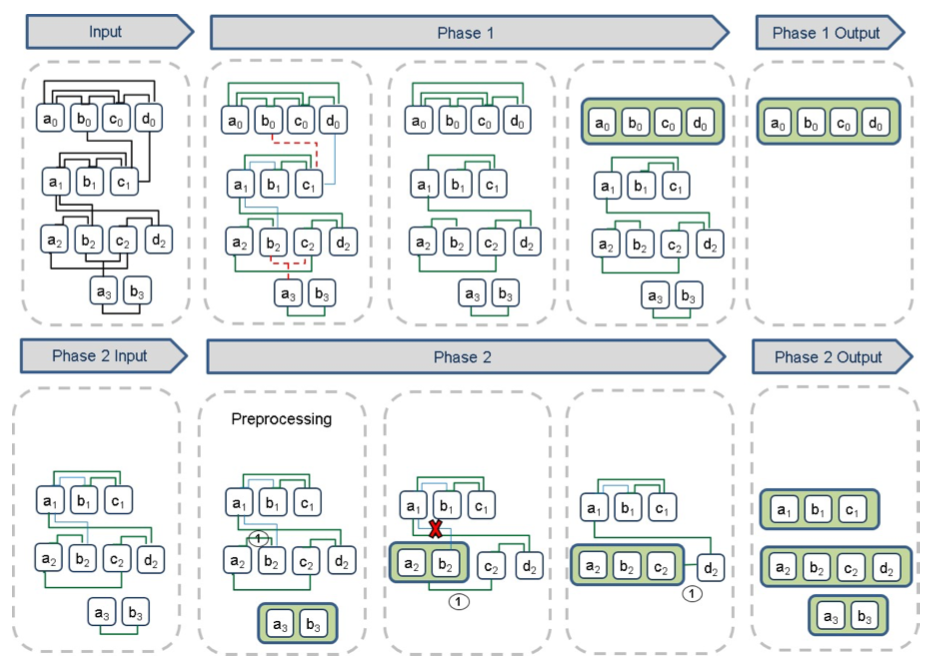
\includegraphics[width=1\textwidth]{clip_example.png} 
\captionof{figure}{Example of CLIP \cite{Saeedi}}
\label{fig:fig1}
\end{center}

Furthermore, the authors also propose RLIP for repairing clusters generated by different clustering schemes. In its first step, the RLIP algorithm also prioritizes strong links among entities within a cluster, and with this solves overlapping clusters by allocating an overlapped entity to a specific cluster. Here, when overlapped entities have strong links to multiple clusters, the algorithm considers the highest association degree\footnote{``The association degree of an entity for a cluster of size k corresponds to the average similarity of the entity to the k − 1 other entities in the cluster."\cite{Saeedi}} to select a cluster. Besides, overlapped entities with no strong links, and entities with only strong links to other overlapped entities are consider singletons \cite{Saeedi}. Additionally, if necessary, it uses CLIP algorithm to fix source-inconsistent clusters.

As part of their evaluation, Saeedi et al. \cite{Saeedi} point out that CLIP surpass in precision and F-measure (test's accuracy) to the other clustering schemes which they studied. Also they indicate that the cluster quality is exceptional because CLIP algorithm does not consider weak links. Additionally, Saeedi et al. remark that RLIP algorithm can improve F-measure for all the studied clustering schemes. And that both algorithms support scalability in large datasets by parallel implementation.

\subsubsection{AppGrouper: Knowledge-graph-based Interactive Clustering Tool for Mobile App Search Results} \cite{Chang}

\subsubsection{Incorporating Knowledge }

\todo{Read and include information from \cite{Wang}}

\subsubsection{Topical Clustering of Search Results}
\cite{Scaiella} contrast/complement with \cite{Schuhmacher}

In: \cite{Elbattah} they mention the study of \cite{Scaiella}: search results clustering (SRC) was endorsed using a representation of texts as graph of concepts or topics. The nodes (topics) represented Wikipedia pages identified by a means of topic annotation applied to search results, and the edges denoted the relatedness among topics. The study proposed an algorithm that used the spectral properties and labels of topics graph. 

\cite{Elbattah} also mentioned the work of \cite{Schuhmacher} as: proposed a graph-based semantic model for representing document content. Their method relied on the use of DBpedia for acquiring knowledge about entities and their semantic relations, then computing a semantic similarity of documents.


\section{Analysis and comparison of presented approaches} \label{analysis}

\section{Discussion} \label{discussion}
\section{Conclusion} \label{conclusion}

%
% ---- Bibliography ----
%
% BibTeX users should specify bibliography style 'splncs04'.
% References will then be sorted and formatted in the correct style.
%
\bibliographystyle{splncs04}
\bibliography{mybibliography}
%
\begin{thebibliography}{8}
\bibitem{Schmitz}
Schmitz, C., Hotho, A., J{\"a}schke, R., Stumme, G.: Content Aggregation on Knowledge Bases Using Graph Clustering. In: Sure, Y., Domingue, J. (eds.) The Semantic Web: Research and Applications. ESWC 2006, LNCS, vol. 4011, pp. 530--544.
Springer, Berlin, Heidelberg (2006). \doi{10.1007/11762256\_39}

\bibitem{Elbattah}
Elbattah, M., Roushdy, M., Aref, M., M.Salem, A.: Large-Scale Entity Clustering Based on Structural Similarity within Knowledge Graphs. In: Arun, K., Somani, G. (eds.) Big Data Analytics: Tools and Technology for Effective Planning, Edition: 1, Chapter: 14, pp. 311--334. CRC Press Editors (2017). \doi{10.1201/b21822-14}

\bibitem{Saeedi}
Saaedi, A., Peukert, E., Rahm, E.  : Using Link Features for Entity Clustering in Knowledge Graphs. In: Gangemi, A., Navigli, R., Vidal, M., Hitzler, P., Troncy, R., Hollink, L., Tordai, A., Alam, M. (eds.) The Semantic Web. ESWC 2018, LNCS, vol. 10843, pp. 576--592.
Springer International Publishing, Cham (2018). \doi{10.1007/978-3-319-93417-4\_37}

\bibitem{Pedrycz}
Pedrycz, W.: Knowledge-Based Clustering: From Data to Information Granules. 2nd edn. Wiley-Interscience, New York, NY, USA (2005)

\bibitem{Zhang}
Zhang, X., Lv, Y., Lin, E : Object Clustering in Linked Data using Centrality. In: Proceedings of China Conference on Knowledge Graph and Semantic Computing (CCKS2016)
on Proceedings, pp. 172--183. Publisher, Location (2016). \doi{10.1007/978-981-10-3168-7\_17}

\bibitem{Ehrlinger}
Ehrlinger, L, W{\"o}{\ss}, W.: Towards a Definition of Knowledge Graphs. In: Martin, M., Cuquet M., Folmer, E. (eds.) In Joint Proceedings of the Posters and Demos Track of the 12th International Conference on Semantic Systems - SEMANTiCS2016 and the 1st International Workshop on Semantic Change \& Evolving Semantics (SuCCESS'16), CEUR-WS, vol. 1695, Leipzig, Germany (2016). \doi{10.10007/1234567890}

\bibitem{Paulheim}
Paulheim, H.: Knowledge Graph Refinement: A Survey of Approaches and Evaluation Methods. Semantic Web Journal, 489--508 (2017). \doi{10.3233/SW-160218}

\bibitem{Farber}
F{\"a}rber, M., Bartscherer, F, Menne,C., Rettinger, A.: Linked data quality of DBpedia, Freebase, OpenCyc, Wikidata, and YAGO. Semantic Web Journal, 77--129 (2018). \doi{10.3233/SW-170275}

\bibitem{Tripathi}
Tripathi, K.: A Review on Knowledge-based Expert System: Concept and Architecture. IJCA Special Issue on Artificial Intelligence Techniques-Novel Approaches \& Practical Applications (2011). \doi{10.5120/2845-226}

\bibitem{Engelmore}
Engelmore R.S.  : Artificial Intelligence and Knowledge Based Systems: Origins, Methods and Opportunities for NDE. In: Thompson D.O., Chimenti D.E. (eds.) Review of Progress in Quantitative Nondestructive Evaluation. Review of Progress in Quantitative Nondestructive Evaluation, vol. 6 A., 
Springer, Boston, MA (1987). \doi{10.1007/978-1-4613-1893-4\_1}

\bibitem{Diestel}
Diestel, R.: Graph Theory. 4th edn. Springer, New York, NY, USA, (2012)

\bibitem{Robinson}
Robinson, I., Webber, J.,Eifrem, E.: Graph Databases. 2nd edn. O'Reilly Media, Inc., Sebastopol, CA (2015)

\bibitem{Pan}
Pan, J., Vetere, G., Gomez-Perez, J., Wu,: Exploiting Linked Data and Knowledge Graphs in Large Organisations. 1st edn. Springer International, Switzerland, (2017)

\bibitem{Zacharski}
Zacharski, R.: A Programmer's Guide to Data Mining. http://guidetodatamining.com/ (2012)

\bibitem{Han}
Han, J., Kamber, M., Pei, J.: Data Mining: Concepts and Techniques. 3rd edn. Morgan Kaufmann Publishers Inc.,
San Francisco, CA, USA (2011)

\bibitem{Mirkin}
Mirkin, B.: Clustering For Data Mining: A Data Recovery Approach. 2nd edn. Chapman \& Hall/CRC,
Boca Raton, FL, USA (2005)

\bibitem{Tang}
Tang, G., Pei, J., Luk, W.: Email Mining: Tasks, Common Techniques, and Tools. Knowl. Inf. Syst., 1--31 (2014). \doi{10.1007/s10115-013-0658-2}

\bibitem{Berkhin}
Berkhin, P.: A Survey of Clustering Data Mining Techniques. In: Kogan, J., Nicholas, C., Teboulle, M. (eds.) Grouping Multidimensional Data: Recent Advances in Clustering 2006, pp. 25--71.
Springer Berlin Heidelberg, Berlin, Heidelberg (2006). \doi{10.1007/3-540-28349-8\_2}

\bibitem{Schaeffer}
Schaeffer, S.: Survey: Graph Clustering. Comput. Sci. Rev., 27--64 (2007). \doi{10.1016/j.cosrev.2007.05.001}

\bibitem{Aggarwal}
Aggarwal, C., Wang, H.: A Survey of Clustering Algorithms for Graph Data. In: Aggarwal, C., Wang, H. (eds.) Managing and Mining Graph Data, pp. 275--301.
Springer US, Boston, MA, USA (2010). \doi{10.1007/978-1-4419-6045-0\_9}

\bibitem{Chang}
Chang, S., Dai, P., Hong, L., Sheng, C., Zhang, T., Chi, E.: AppGrouper: Knowledge-based Interactive Clustering Tool for App Search Results. In: Proceedings of the 21st International Conference on Intelligent User Interfaces, pp. 348--358. ACM, New York, NY, USA (2016) \doi{10.1145/2856767.2856783}

\bibitem{Carpineto}
Carpineto, C., Osi\'{n}ski, S, Romano, G., Weiss, D. : A Survey of Web Clustering Engines. ACM Comput. Surv., 17:1--17:38 (2009)

\bibitem{Wang}
Wang, C., Song, Y., El-Kishky, A., Roth, D. and Zhang, M., Han, J.: Incorporating World Knowledge to Document Clustering via Heterogeneous Information Networks. In: Proceedings of the 21th ACM SIGKDD International Conference on Knowledge Discovery and Data Mining, pp. 1215--1224. ACM, New York, NY, USA (2015)

\bibitem{Scaiella}
Scaiella, U., Ferragina, P., Marino, A., Ciaramita, M.: Topical Clustering of Search Results. In: Proceedings of the Fifth ACM International Conference on Web Search and Data Mining, pp. 223--232. ACM, Seattle, Washington, USA (2012) \doi{10.1145/2124295.2124324}

\bibitem{Schuhmacher}
Schuhmacher, M., Ponzetto, S.: Exploiting DBpedia for Web Search Results Clustering. In: Proceedings of the 2013 Workshop on Automated Knowledge Base Construction, pp. 91--96. ACM, San Francisco, California, USA (2013) \doi{10.1145/2509558.2509574}

\bibitem{Huang}
Huang, Z.: Data Mining and Knowledge Discovery. Database Management \& Information Retrieval 22--83 (1998) \doi{10.1023/A:1009769707641} 

\bibitem{Peukert}
Saeedi, A., Peukert, E., Rahm, E.: Comparative Evaluation of Distributed Clustering Schemes for Multi-source Entity Resolution. In: Kirikova M., N\o rv\aa g K., Papadopoulos G. (eds.), ADBIS 2017, LNCS, vol. 10509, pp. 278--293. Springer International (2017). \doi{10.1007/978-3-319-66917-5\_19}

\end{thebibliography}

\begin{comment}
\bibitem{ref_lncs1}
Author, F., Author, S.: Title of a proceedings paper. In: Editor,
F., Editor, S. (eds.) CONFERENCE 2016, LNCS, vol. 9999, pp. 1--13.
Springer, Heidelberg (2016). \doi{10.10007/1234567890}

\bibitem{ref_article1}
Author, F.: Article title. Journal \textbf{2}(5), 99--110 (2016)

\bibitem{ref_book1}
Author, F., Author, S., Author, T.: Book title. 2nd edn. Publisher,
Location (1999)

\bibitem{ref_proc1}
Author, A.-B.: Contribution title. In: 9th International Proceedings
on Proceedings, pp. 1--2. Publisher, Location (2010)

\bibitem{ref_url1}
LNCS Homepage, \url{http://www.springer.com/lncs}. Last accessed 4
Oct 2017

\end{comment}
\end{document}


